% !TEX root = catron-dissertation.tex
\epstopdfsetup{outdir=./images/01_introduction/}

\chapter{Introduction}
\label{chap:01_intro}

There have been two major attempts to field a directed-energy system aboard an aircraft to date \cite{Jumper-2013-8KtN3pue}.
The first was the Airborne Laser Laboratory (ALL) which took place in the late 1970's and early 1980's which used a CO$_2$ laser with a wavelength of 10.6-$\mu$m.
The second was the Airborne Laser (ABL) program which operated in the 2000's and used a COIL laser at 1.315-$\mu$m.
Airborne optical systems like ALL and ABL have to deal with a phenomenon known as ``aero-optics,'' which refers to optical distortions caused by compressible aero-dynamic flow features that pass through the outgoing beam.
These optical distortions were first noticed due to image degradation in wind tunnel measurements in the 1950's \cite{Stine-1956-UaRzVZCe} as well as in photo-reconnaissance missions in the 1960's \cite{Kyrazis-2013-vwKeEBym}.

The peak on-target irradiance of a beam passing through an optical disturbance, $I$, divided by the diffraction-limited performance, $I_0$, is known as the Strehl ratio \cite{Mahajan-1982-kkXM4eaB}, $\sr$,
\begin{equation}
  \sr = \frac{I}{I_0} \textrm{.}
  \label{eqn:01_strehl_ratio_definition}
\end{equation}
The diffraction-limited performance is the beam intensity that would exist on the same target if not for the optical disturbance.
The Airborne Laser Laboratory had an estimated Strehl ratio of 95\%\cite{Jumper-2013-8KtN3pue} so that the ``aero-optics problem'' effectively did not apply for this case.
Following the Airborne Laser Laboratory program there was a desire to move toward shorter wavelengths in order to take advantage of improved diffraction-limited performance, leading to a smaller-diameter focused spot on target with a higher irradiance $I_0$: \cite{Jumper-2001-6QDh7zDy},
\begin{equation}
  \frac{I_0}{P} = \frac{1}{\pi}\left(\frac{Ap}{\lambda z}\right)^2 \textrm{,}
  \label{eqn:01_farfield_intensity}
\end{equation}
where $P$ is the laser output power, $Ap$ is the aperture size, and $z$ is the propagation distance.
The improvement in diffraction-limited performance as the laser wavelength is decreased is shown in Figure \ref{fig:01_farfield_intensity}.
\begin{figure}
  \centering
  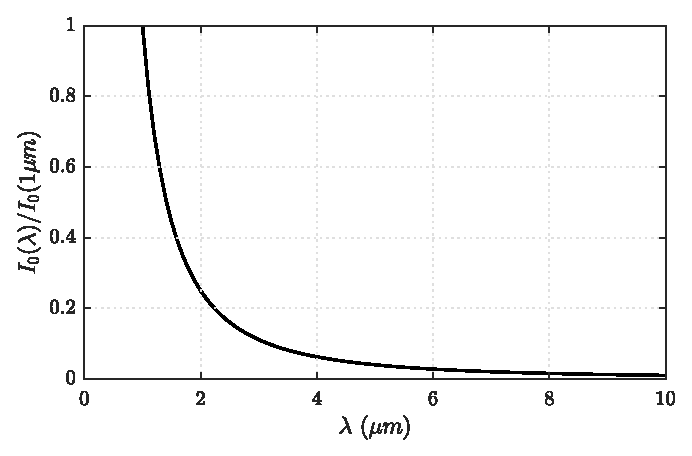
\includegraphics{../matlab/01_introduction/farfield_intensity.eps}
  \caption{Diffraction-limited far-field intensity of a beam normalized by the performance at 1-$\mu$m.}
  \label{fig:01_farfield_intensity}
\end{figure}
By only changing the laser source from a 10-$\mu$m to 1-$\mu$m wavelength the diffraction-limited performance can be increased 100 times.

Aero-optical issues start to become important as the wavelength is decreased as is evident from the Mar\'echal approximation \cite{Mahajan-1983-hg7ahvJM} which relates the Strehl ratio to wavelength,
\begin{equation}
  \sr \approx \exp\left\{-\left[\frac{2\pi \opdrms}{\lambda}\right]^2\right\} \textrm{,}
  \label{eqn:01_strehl_ratio}
\end{equation}
where $\opdrms$ is the spatial root-mean-square of the optical path difference over the aperture and is a way to quantify the optical disturbance as will be discussed further in Chapter \ref{chap:02_lit_review}.
As stated above, the ALL had a Strehl ratio of 95\%; however, if the ALL system's laser was swapped with another laser of a lower wavelength, the Strehl ratio would significantly decrease as shown by Figure \ref{fig:01_strehl_ratio}.
\begin{figure}
  \centering
  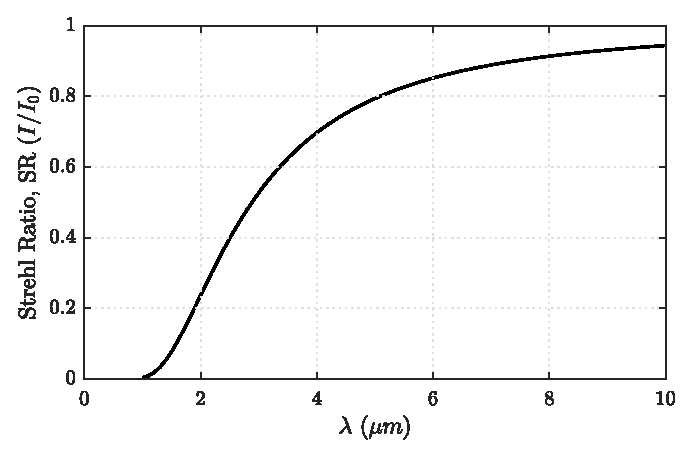
\includegraphics{../matlab/01_introduction/strehl_ratio.eps}
  \caption{Strehl ratio due to the $\opdrms$ of the Airborne Laser Laboratory (ALL) at various laser wavelengths.  ALL had an estimated Strehl ratio of 95\% with its 10.6-$\mu$m laser.}
  \label{fig:01_strehl_ratio}
\end{figure}
While going from 10 to 1-$\mu$m hypothetically results in a 100-fold increase in diffraction-limited performance, the actual on-target intensity that this hypothetical system obtains would be essentially zero due to the much larger effect that aero-optical aberrations have on the outgoing beam as the wavelength is reduced.
This means that the aero-optical problem can no longer be ignored, which was recognized as one of the main developmental risks of the ABL program \cite{DOTE-1999-HnkadUEw}.

As the next generation of airborne directed-energy systems are developed some amount of ground testing of those systems will need to occur.
In order to understand the aero-optical environment that these systems will experience in the air, wind tunnel tests will need to be employed.
These tests are cheaper to perform than, for example, flight testing, and allow for quicker iteration of design parameters.
However, as will be described in further detail in Chapter \ref{chap:02_lit_review}, wind-tunnel measurements of aero-optical effects typically require passing a test beam into and through the test-section, so that the test beam is susceptible to acquiring additional optical contamination including but not limited to the boundary layer present on the wall and the acoustic environment generated by the wind tunnel fan \cite{Gordeyev-2014-jcJndkHM}.
Note that it is common in signal-processing terminology to use the word “noise” to describe unwanted interference that appears in addition to the “signal” that is the objective of the measurement; however, in this dissertation, the word “contamination” is used to describe any optical noise sources that are unrelated to the aero-optical signal, in order to avoid confusion with use of the word “noise” to describe acoustic noise which, as will be shown, is also a source of optical contamination.

Assuming that the optical disturbances from aero-optical effects are statistically independent from the contaminating optical disturbances from the testing environment, we can estimate the total optical disturbance as
\begin{equation}
  \opdrms_{TOTAL}^2 = \opdrms_{MODEL}^2+\opdrms_{ENVIRONMENT}^2 \textrm{.}
  \label{eqn:01_combined_opd}
\end{equation}
As an example of the effect that optical contamination may have on system design, Figure \ref{fig:01_design_iteration} illustrates a hypothetical iterative design process, where the design objective is to obtain a design that meets a required level of performance shown in red, in the presence of a level of environmental optical contamination shown in orange.
\begin{figure}
  \centering
  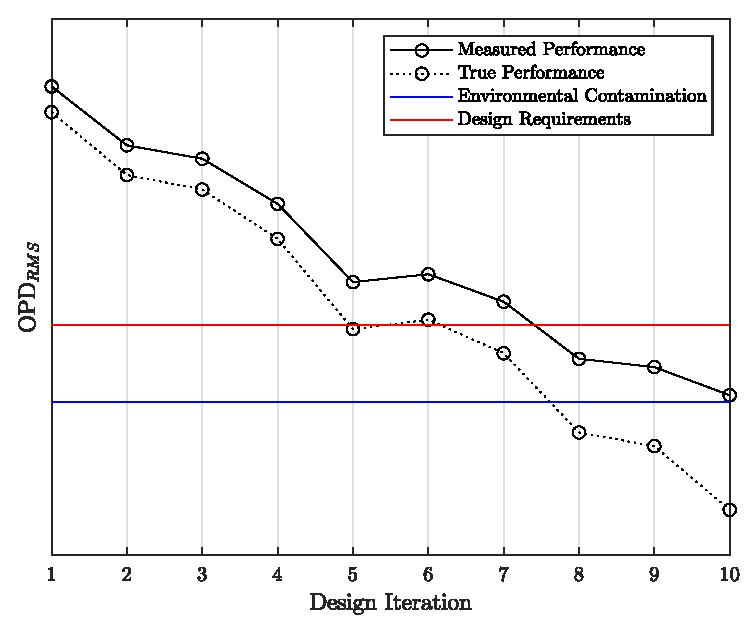
\includegraphics{../matlab/01_introduction/design_iteration.eps}
  \caption{Hypothetical iterative design process of an airborne directed-energy system.  The required performance level is shown by the red line and the testing environment's contamination is shown by the orange line.}
  \label{fig:01_design_iteration}
\end{figure}
The design process was simulated by an initial aero-optical $\opdrms$ shown on the left of the plot, and the improvement in system performance achieved with each design iteration was simulated as a nearly linear reduction in $\opdrms$ combined with 15\% random variation.
If only the measured data, that is, including the effect of environmental contamination using Equation \ref{eqn:01_combined_opd}, is used to assess the system's performance then three additional design iterations are needed to achieve a usable design, which can add significantly to the development time and costs.
If the environmental contamination is greater than the design requirement, the measured performance will never reach the required performance criteria.
However, if the environmental contamination can be estimated, mitigated and/or removed, then the measured performance is a more accurate evaluation of the true aero-optical performance, and design convergence can be achieved more quickly and with more accurate results.

This dissertation will examine the environmental contamination of aero-optical measurements in wind tunnels, with a particular focus on the contamination due to acoustic noise within the wind tunnel.
A review of the available literature and important concepts in given in Chapter \ref{chap:02_lit_review}.
In Chapter \ref{chap:03_optical_acoustics}, the optical disturbances caused by acoustic waves from simple plane and spherical waves are presented, leading to a process for estimating the acoustical environment within the test section of a wind tunnel.
The strength of an spherical acoustic wave will be assessed with both microphone and optical measurements.
Multi-dimensional spectral techniques will be used to analyze optical wavefronts in Chapter \ref{chap:04_dispersion} and to filter optical wavefronts in Chapter \ref{chap:06_single_filter}.
These filtering techniques will contain some optical contamination particularly in regions where the various signal components interfere with one another.
In order to further reduce the optical contamination, Chapter \ref{chap:07_multiple_filter} will utilize additional sensor information from both microphones and accelerometers to remove some of the overlapping contamination to obtain a better picture of the actual optical performance of an airborne directed-energy system from ground test measurements.
